\documentclass[a4paper, 12pt]{article}

\usepackage{wrapfig}
\usepackage{graphicx}
\usepackage{mathtext}
\usepackage{amsmath}
\usepackage{siunitx}
\usepackage{subfigure}
\usepackage{multirow}
\usepackage{rotating}
\usepackage[T1,T2A]{fontenc}
\usepackage[russian]{babel}
\usepackage{caption}

\graphicspath{{pictures/}}


\title{\begin{center}Лабораторная работа №2.4.1\end{center}
Определение теплоты испарения жидкости}
\author{Гёлецян А.Г.}
\date{\today}

\begin{document}
    \pagenumbering{gobble}
    \maketitle
    \newpage
    \pagenumbering{arabic}


    \textbf{Цель работы:} 1) измерение давления насыщенного пара жидкости при разной температуре; 2) вычисление по полученным данным теплоты испарения с помощью уравнения Клапейрона-Клаузиуса.

    \textbf{В работе используются:} термостат, герметический сосуд, заполненный водой, отсчётный микроскоп.


    \section{Теоретическая часть}
    \subsection{Уравнение Клапейрона-Клаузиуса}
    Если считать что насыщенные пары подчиняются закона Менделеева-Клапейрона, и пренебречь удельным объемом жидкости относительно удельного объема паров то из уравнения Клапейрона-Клаузиуса получаем формулу для удельной теплоты испарения

    \begin{equation}\label{L}
        L = \frac{RT^2}{\mu P}\frac{dP}{dT} = - \frac{R}{\mu} \frac{d(ln P)}{d(1/T)}
    \end{equation}

    Как видим, если измерить зависимость давления насыщенных паров от температуры по формуле (\ref{L}) можно получить удельную теплоту испарения.
    \subsection{Экспериментальная установка}
    \begin{figure}[h]
        \center{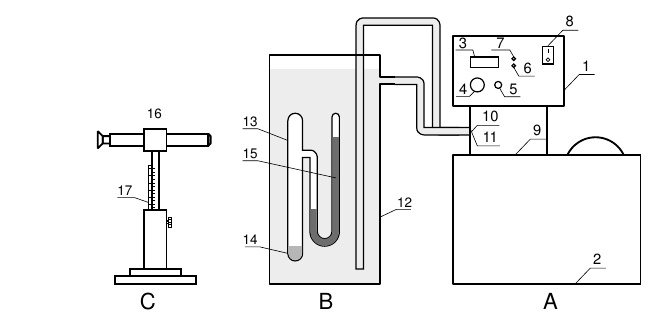
\includegraphics[width=\textwidth]{ustanovka}}
        \caption{Установка для определения давления насыщенных паров.}
        \label{ustanovka}
    \end{figure}
    \paragraph{}
    Измерения проводятся на установке, изображенной на рис. \ref{ustanovka}. С помощью термостата A выставляется желаемя температура, и с помощью микроскопа C измеряется положение менисков ртути в U-образном монометре 15. Давление насыщенных паров считается как разность высот менисков ртути.
    \paragraph{}
    Измерения проводятся в 2 этапа. В начале жидкость нагревается, а потом остужается. Это делается для того, чтобы посмотреть зависит ли давление насыщенных паров только от состояния жидкости или нет.

    \section{Измерения}
    Измеряем давление по вышеописанной схеме в диапазоне температур от 22 до 37 $^\circ C$. Получаем следующие данные

    \begin{table}[h!]
        \vspace{5pt}
        \begin{center}
        \subtable
        {
            \begin{tabular}{|l|rrr|r|}
            \hline
            № &    $T, ^\circ C$ &    $h_1, см$ &  $h_2, см$ & $Н$ \\
            \hline
            0  &  24.09 &  7.900 &  5.950 &     1 \\
            1  &  25.08 &  7.990 &  5.895 &     1 \\
            2  &  26.06 &  8.050 &  5.840 &     1 \\
            3  &  27.05 &  8.125 &  5.765 &     1 \\
            4  &  28.07 &  8.195 &  5.695 &     1 \\
            5  &  29.08 &  8.305 &  5.595 &     1 \\
            6  &  30.06 &  8.390 &  5.520 &     1 \\
            7  &  31.04 &  8.500 &  5.445 &     1 \\
            8  &  32.07 &  8.610 &  5.340 &     1 \\
            9  &  33.04 &  8.700 &  5.250 &     1 \\
            10 &  34.06 &  8.815 &  5.150 &     1 \\
            11 &  35.04 &  8.910 &  5.040 &     1 \\
            \hline
            \end{tabular}
        }
        \subtable
        {
            \begin{tabular}{|l|rrr|r|}
            \hline
            № &    $T, ^\circ C$ &    $h_1, см$ &  $h_2, см$ & $Н$ \\
            \hline
            12 &  36.06 &  9.045 &  4.930 &     1 \\
            13 &  37.05 &  9.175 &  4.720 &     1 \\
            14 &  38.00 &  9.290 &  4.720 &     1 \\
            15 &  35.86 &  9.090 &  4.895 &     0 \\
            16 &  33.94 &  8.880 &  5.085 &     0 \\
            17 &  32.00 &  8.680 &  5.280 &     0 \\
            18 &  29.97 &  8.455 &  5.475 &     0 \\
            19 &  28.00 &  8.290 &  5.610 &     0 \\
            20 &  26.00 &  8.130 &  5.770 &     0 \\
            21 &  24.01 &  7.970 &  5.890 &     0 \\
            22 &  21.88 &  7.770 &  6.085 &     0 \\
            \hline
            \end{tabular}
        }

        \caption{Измеренные положения менисков в зависимости от температуры.}
        \label{data_raw}
        \end{center}
    \end{table}

    В таблице (\ref{data_raw}) $h_1$ и $h_2$ это координаты правого и левого мениска соответственно относительно некоторой точки. Для ошибок измерения имеем следующее
    \begin{align*}
        \Delta h &= 0.005см\\
        \Delta T &= 0.01К
    \end{align*}
    Заметим, что ошибка температуры $\Delta T$ это ошибка в значениях термометра, который измеряет температуру воды в термостате. Температура воды в балоне может отличатся от температуры воды в ванне. Столбец Н равен 1 если измерение проводились в цикле нагрева и 0 если в цикле охлаждения.
    \paragraph{}
    Если посмотреть на данные внимательно, можно заметить что $h_1 + h_2$ не остается константой, что на первый взгляд может показатся странным, и может намекнуть на недостатучную точность в эксперименте. Для исследования этого вопроса построим график зависимости $h_1+h_2$ от $h_1$.

    \begin{figure}[h]
        \center{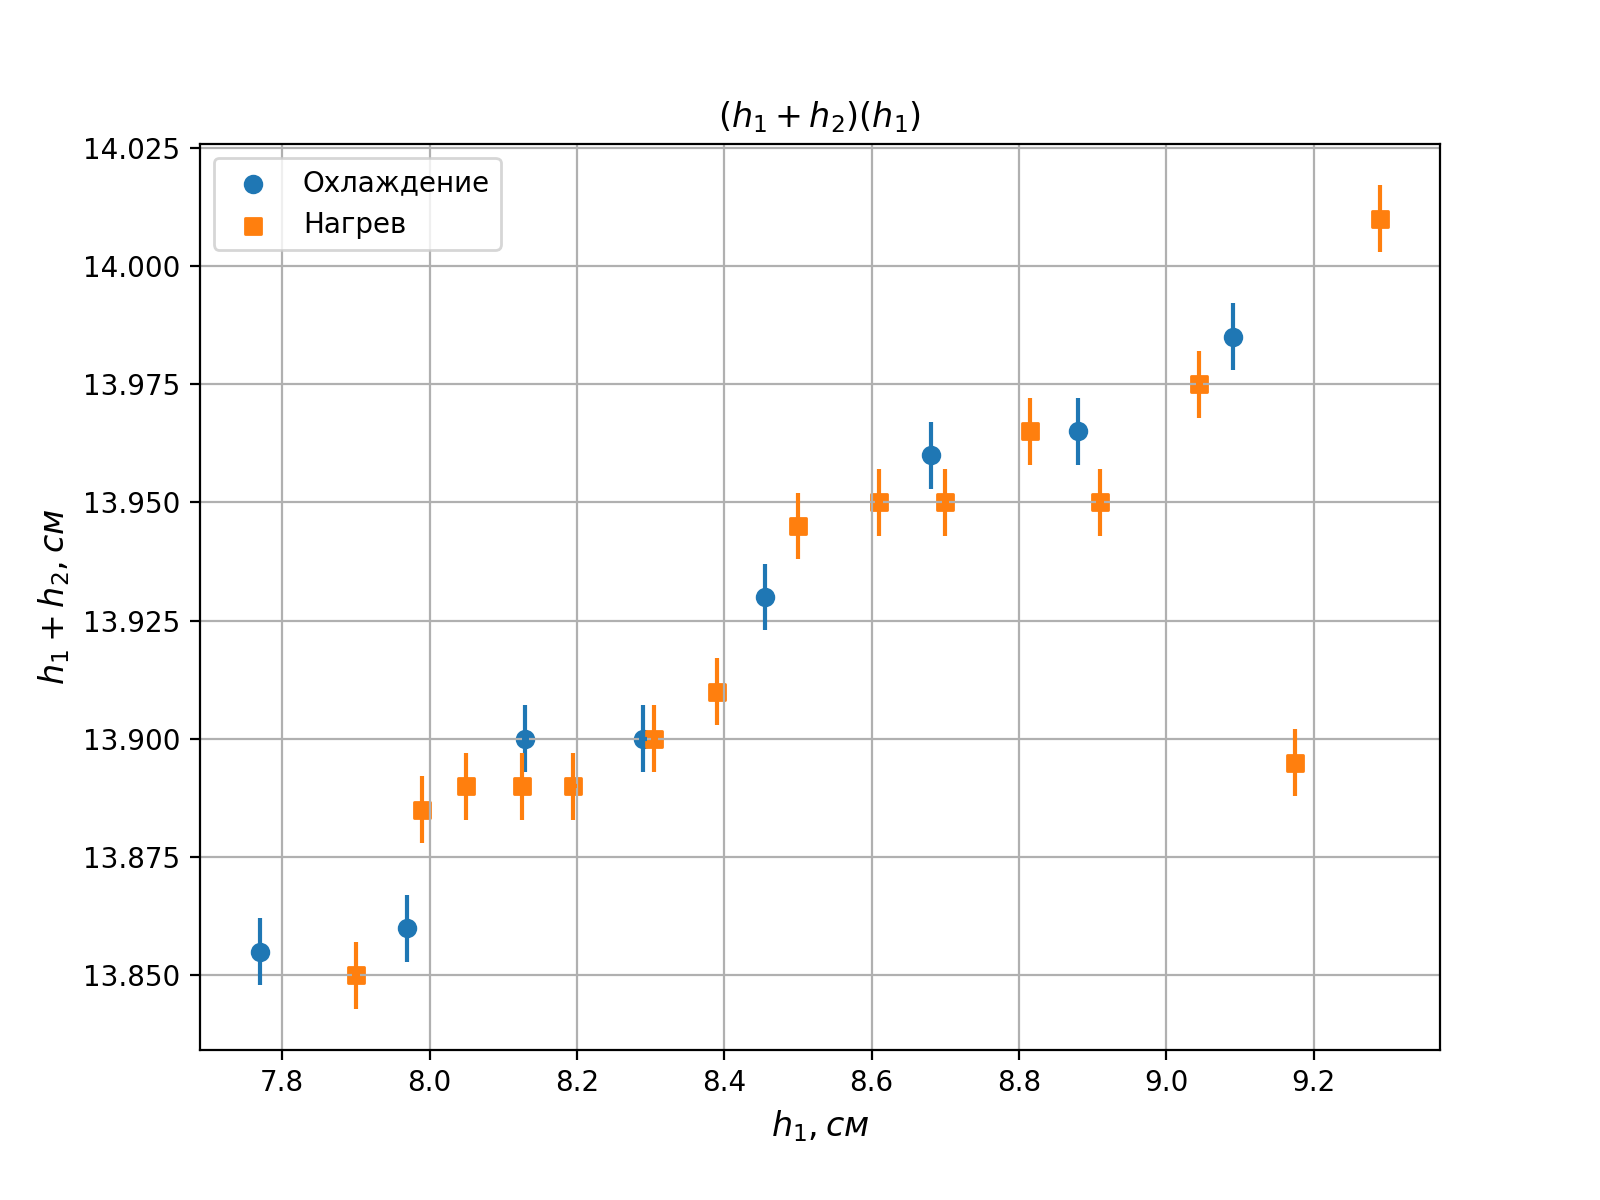
\includegraphics[width=\textwidth]{H(h)}}
        \caption{Зависимость $(h_1+h_2)(h_1)$.}
        \label{H(h)}
    \end{figure}
    Как видим, при нагреве и охлаждении при близких значениях $h_1$ $h_1 + h_2$ почти равны. Это свидетеьствует о том, что все таки точности в эксперименте хватает, и изменение $h_1+h_2$ скорее является следствием других факторов, а не результатом неточных измерении. Единственная странная точка это точка $№ 13$, но во всем остальном все хорошо.

    \paragraph{}
    Теперь, когда разобрались с этим вопросом, считаем давление паров при разных температурах.
    \begin{table}[h!]
        \vspace{5pt}
        \begin{center}
        \subtable
        {
            \begin{tabular}{|l|rr|r|}
            \hline
            № &    $T, ^\circ C$ & $P, торр$ & $Н$ \\
            \hline
            0  &  24.09 &  19.50 &     1 \\
            1  &  25.08 &  20.95 &     1 \\
            2  &  26.06 &  22.10 &     1 \\
            3  &  27.05 &  23.60 &     1 \\
            4  &  28.07 &  25.00 &     1 \\
            5  &  29.08 &  27.10 &     1 \\
            6  &  30.06 &  28.70 &     1 \\
            7  &  31.04 &  30.55 &     1 \\
            8  &  32.07 &  32.70 &     1 \\
            9  &  33.04 &  34.50 &     1 \\
            10 &  34.06 &  36.65 &     1 \\
            11 &  35.04 &  38.70 &     1 \\
            \hline
            \end{tabular}
        }
        \subtable
        {
            \begin{tabular}{|l|rr|r|}
            \hline
            № &    $T, ^\circ C$ & $P, торр$ & $Н$ \\
            \hline
            12 &  36.06 &  41.15 &     1 \\
            13 &  37.05 &  44.55 &     1 \\
            14 &  38.00 &  45.70 &     1 \\
            15 &  35.86 &  41.95 &     0 \\
            16 &  33.94 &  37.95 &     0 \\
            17 &  32.00 &  34.00 &     0 \\
            18 &  29.97 &  29.80 &     0 \\
            19 &  28.00 &  26.80 &     0 \\
            20 &  26.00 &  23.60 &     0 \\
            21 &  24.01 &  20.80 &     0 \\
            22 &  21.88 &  16.85 &     0 \\
            \hline
            \end{tabular}
        }

        \caption{Измеренные давления в зависимости от температуры.}
        \label{data}
        \end{center}
    \end{table}

    \begin{figure}[h]
        \center{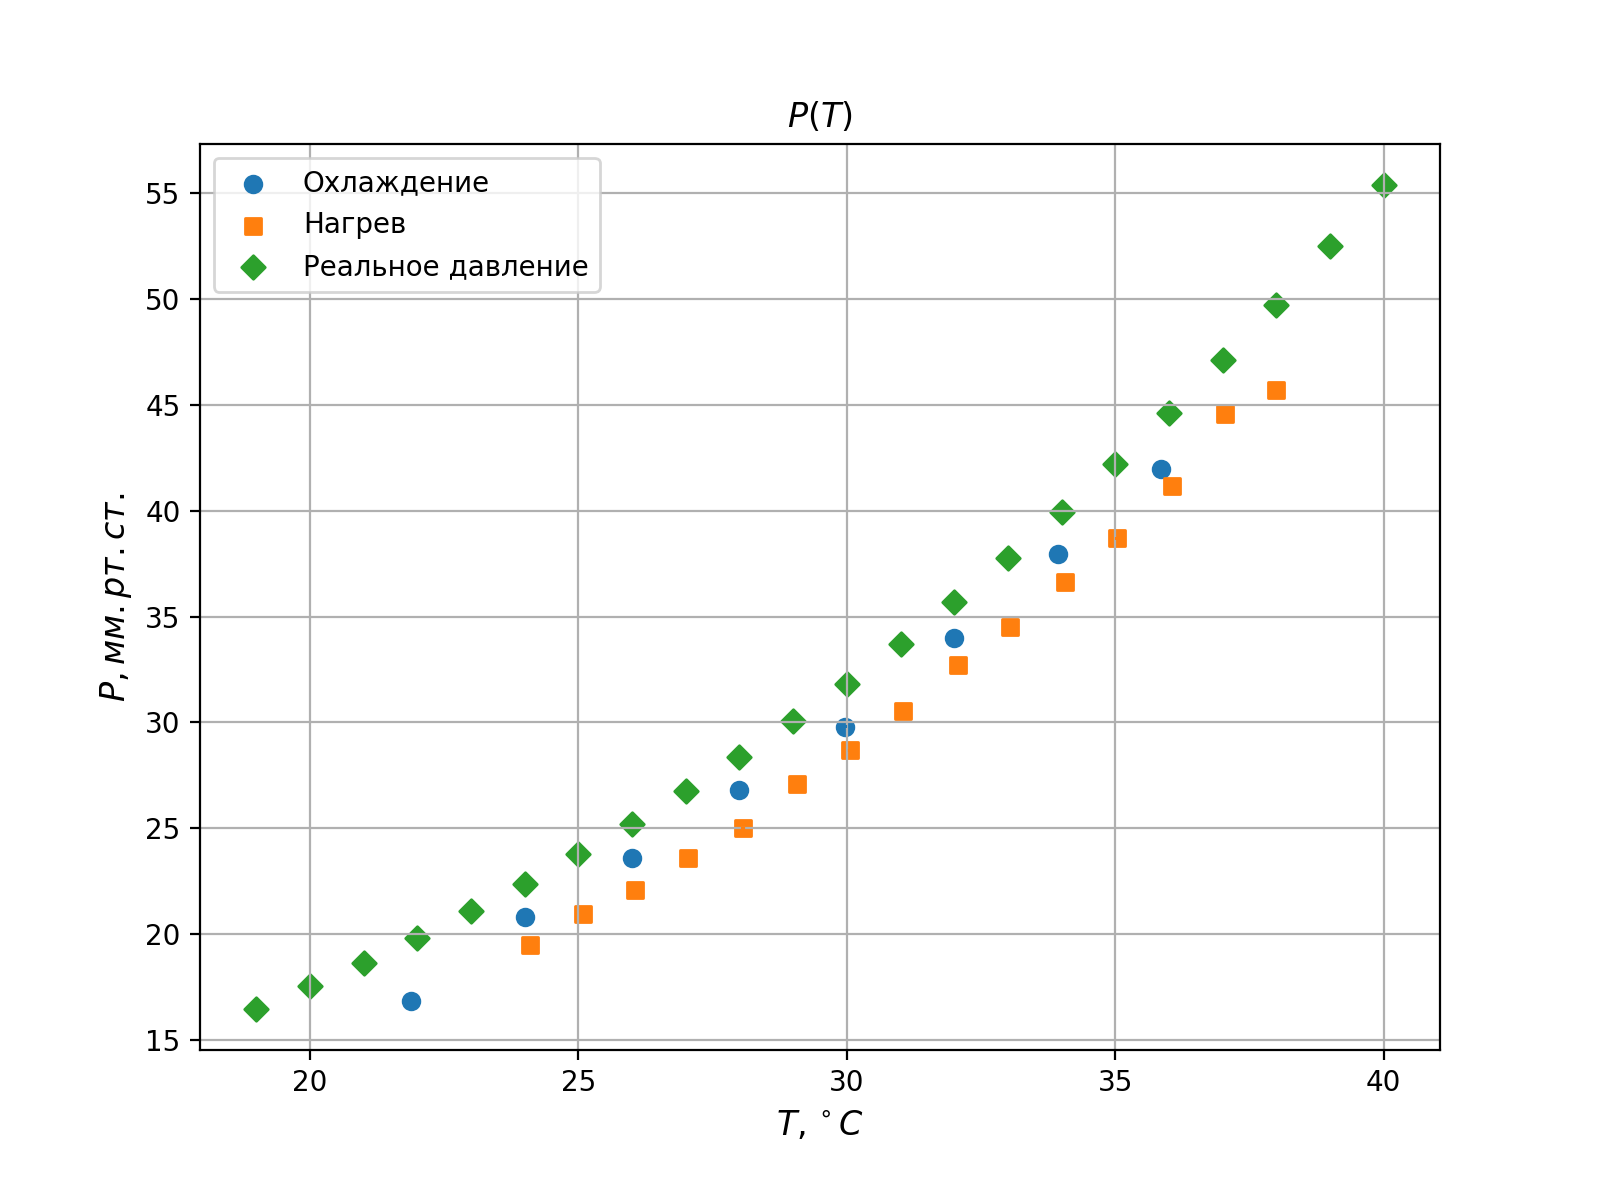
\includegraphics[width=0.8\textwidth]{P(T)}}
        \caption{Зависимость давления насыщенных паров от температуры.}
        \label{P(T)}
    \end{figure}

%     \begin{figure}[h]
%         \center{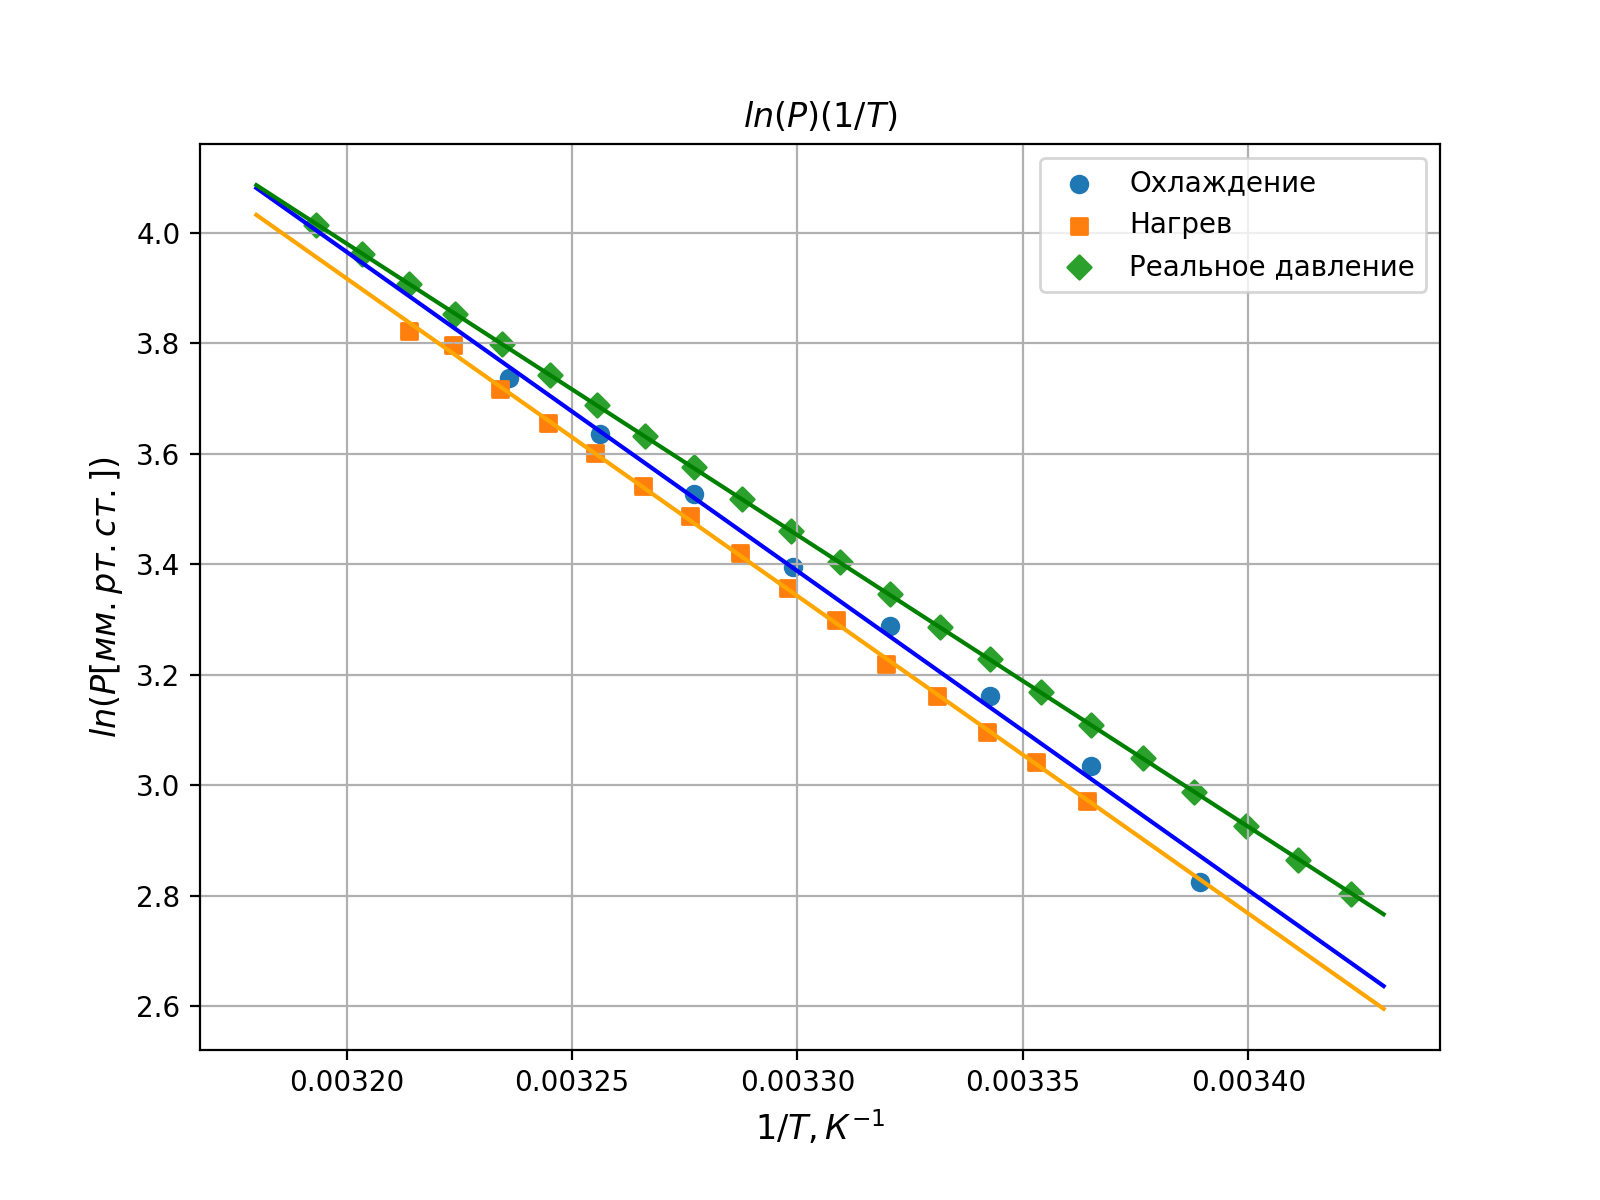
\includegraphics[width=0.8\textwidth]{lnP}}
%         \caption{Зависимость $ln(P) (1/T)$.}
%         \label{lnP}
%     \end{figure}
    Из графика видно, что синие точки смещены влево, что свидетеьствует о том, что во время цикла охлаждения на релаксацию системы не было уделено достаточно времени. Действительно, во время опыта температура жидкости поднималсь на $1 ^\circ C$ примерно каждые 7-10 минут, в то время как жидкость охлаждался на $2 ^\circ C$ примерно каждые 2-4 минут.

    Теперь, для нахождения теплоты испарения построим график зависимости $ln(P) (1/T)$. В предположении что теплота испарения не зависит от температуры эта зависимость имеет вид прямой, а теплота испарения считается по формуле (\ref{L}). Как видим на рис. 4, для оранжевых точек линейная зависимость довольно хорошая, в отличии от синих точек. Объяснение этому дано выше. Аппроксимируя оранжевые, синие и зеленые точки методом МНК имеем следующее

    \begin{align}
        \left(\frac{d(lnP)}{d(1/t)}\right)_{охл.} &= (-5780 \pm 360) К \\
        \left(\frac{d(lnP)}{d(1/t)}\right)_{нагр.} &= (-5750 \pm 90) К\\
        \left(\frac{d(lnP)}{d(1/t)}\right)_{реал.} &= (-5279 \pm 6) К
    \end{align}

    Как видим, в цикле охлаждения ошибки большие, поэтому теплоту испарения будем считать для цикла нагревания. Получаем

    \begin{align}
        L &= (2650 \pm 40)кДж/кг\\
        L_{реал.} &= (2437 \pm 3)кДж/кг
    \end{align}

    \section{Выводы}
    Сравним наши данные с табличными. При $100 ^\circ C$ теплота испарения $L_{100^\circ C}=2256кДж/кг$. Как видим, различия большие. Теперь сравним с теплотой испарения при $30 ^\circ C$ - $L_{30 ^\circ C}=2430кДж/кг$. Как видим, довоьго близко к $L_{реал.}$, что свидетельствует о том что на нашем диапазоне температур формулой (\ref{L}) можно пользоваться. Несмотря на это, мы получили значение $L$, которое отличается от действительного на $\varepsilon_L = 9\%$, что не входит в диапазон погрешности $L$. Причиной всему этому скорее всего является недостаточное время отведенное для релаксации системы, изи за чего действительная температура в балоне ниже регистрируемого. Именно в следствии этих искажении мы и получаем ошибочное значение $L$.



    \begin{sidewaysfigure}
        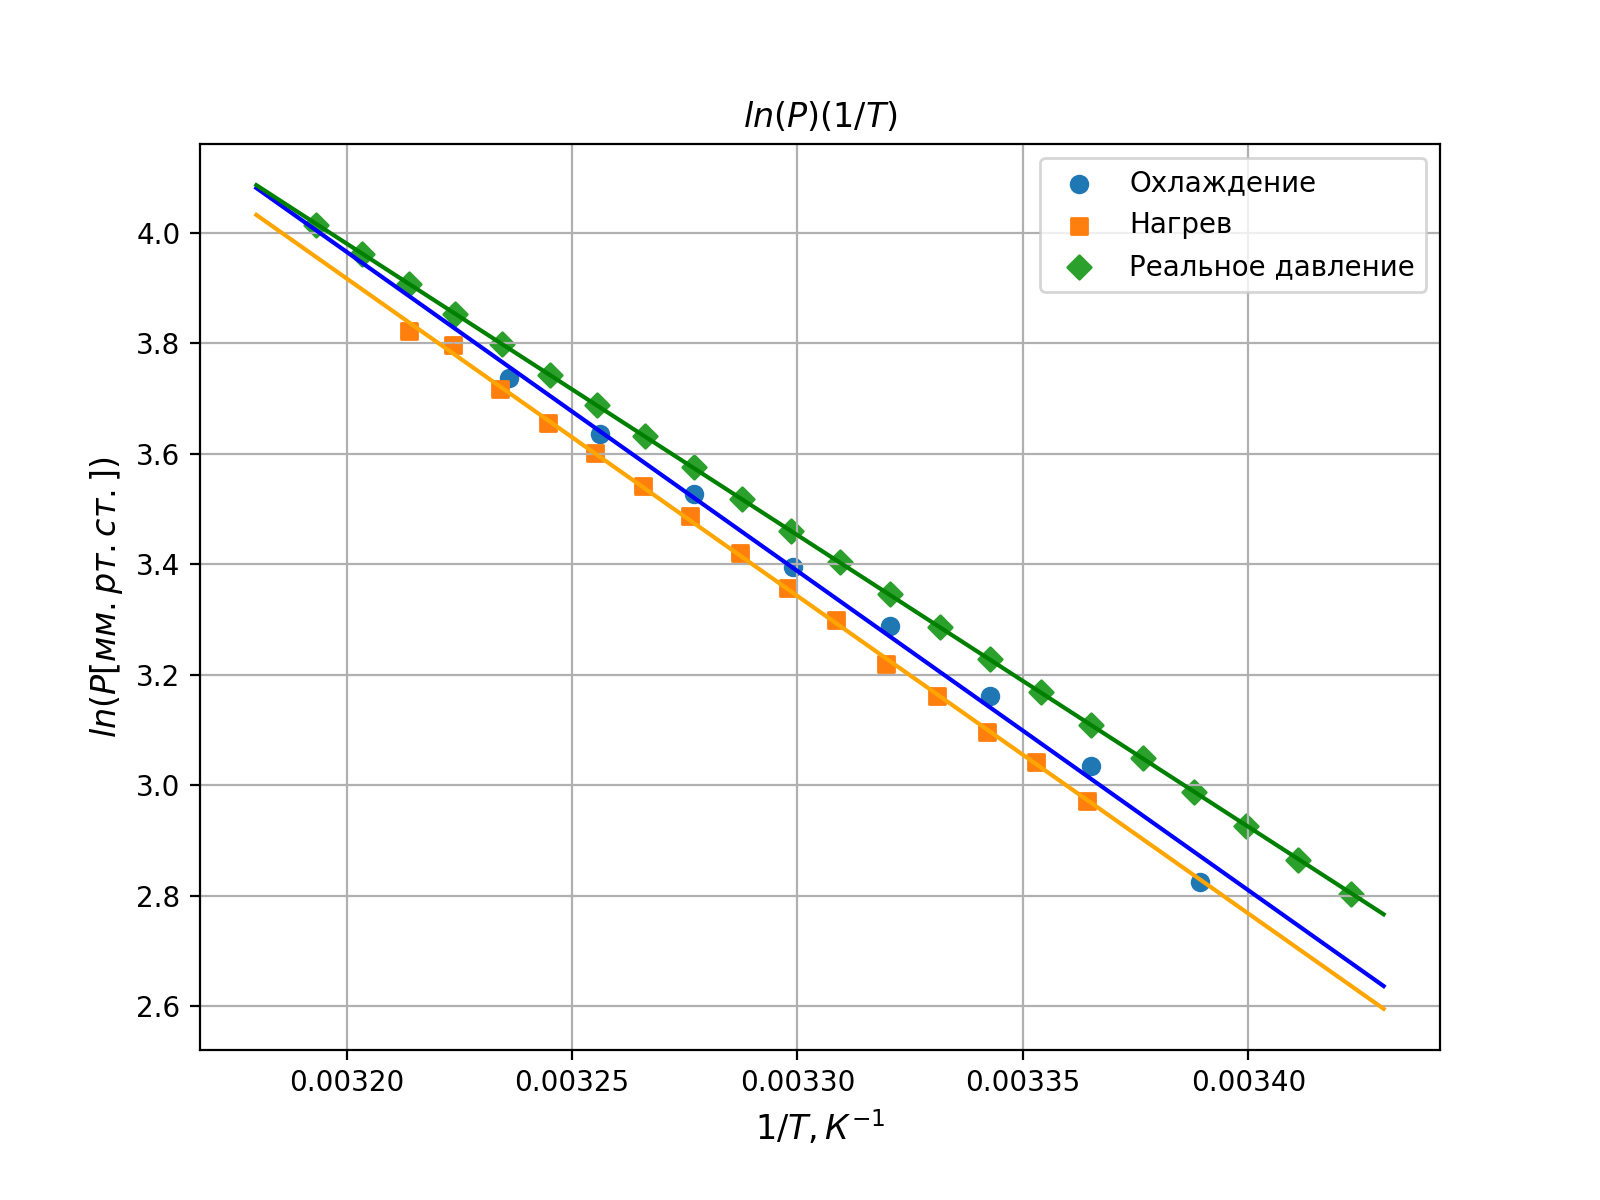
\includegraphics[width=1\textwidth]{lnP}
        \label{lnP}
        \caption{Зависимость $ln(P) (1/T)$.}
    \end{sidewaysfigure}
\end{document}



